\subsection{Layers}
\label{sec:layers}

%\nancomment{could remove archival size from all sections}
We start by analyzing layers in terms of size and compressibility, and file and directory
counts and directory depths.

%%%%%%%%%%%%%%%%%%%%%%%%%%%%%%%%%%%%%%%%%%%%%%%%%%%%%%%%%%%%%%%%%%%%%

\begin{figure}[!t]
	\centering
	\subfigure[CDF of layer sizes]{\label{fig_layer_size_cdf}
		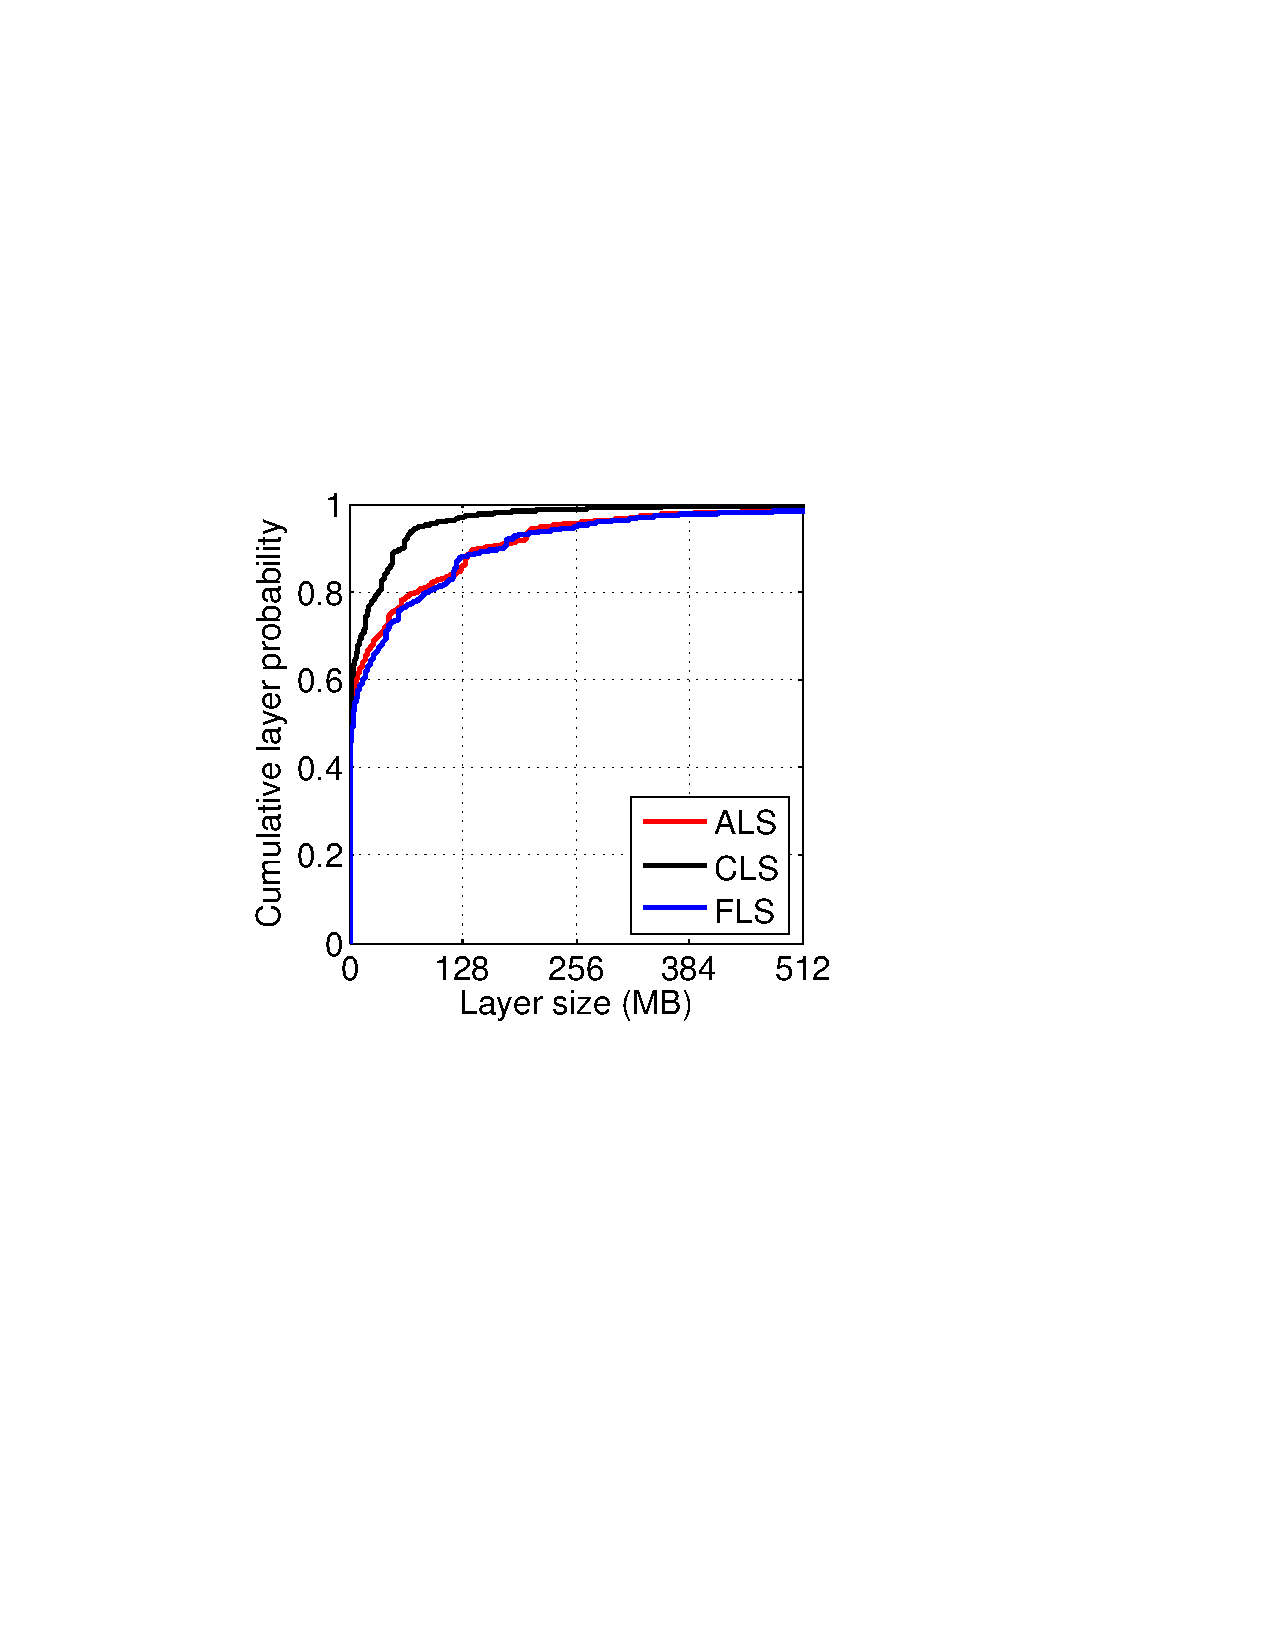
\includegraphics[width=0.234\textwidth]{graphs/layer_size_mb.pdf}
	}
	\subfigure[Histogram of layer sizes]{\label{fig_hist_layer_size}
		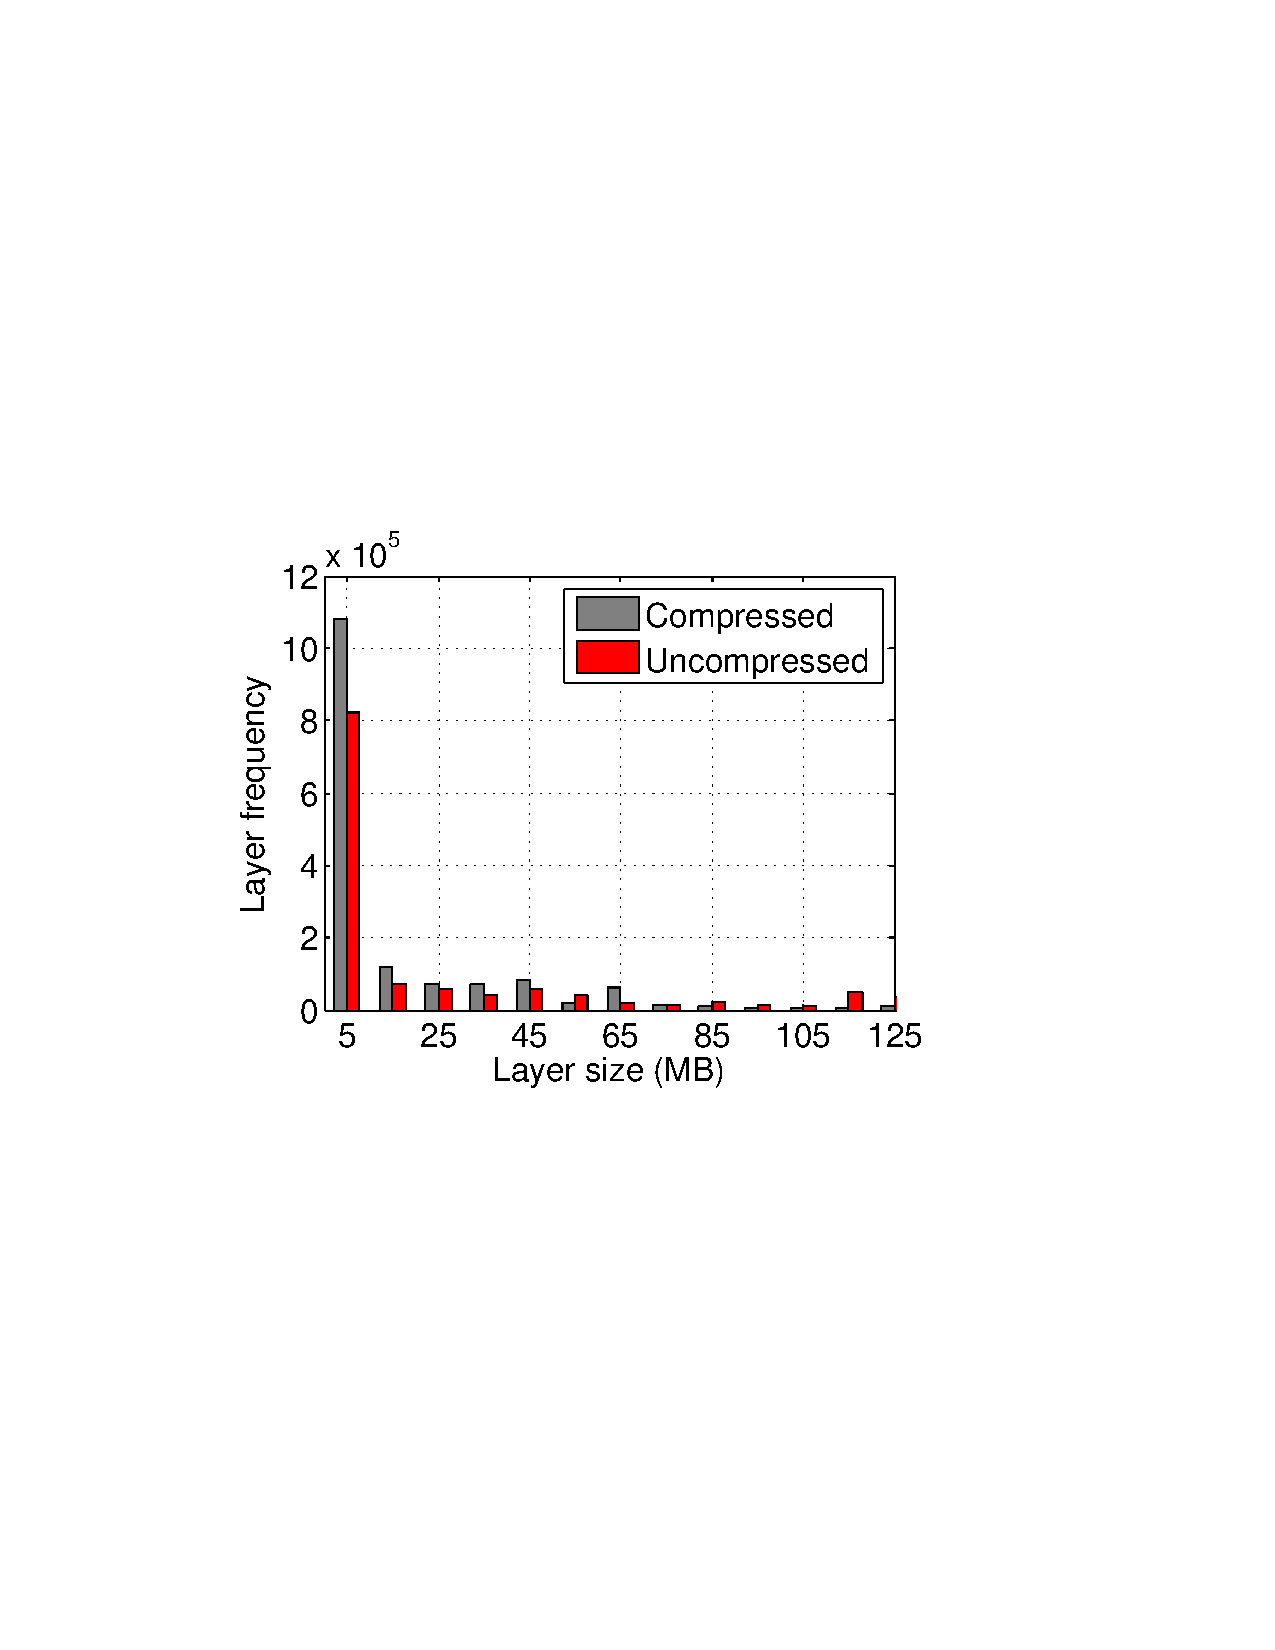
\includegraphics[width=0.213\textwidth]{graphs/hist_layer_size.pdf}
	}
	\caption{Layer size distribution
	\vcomment{Let's use CLS, ALS, and FLS abreviations\nancomment{addressed}}.
	\vcomment{CLS size should go first}.
	\vcomment{We need to use different types of lines (solid, dotted, etc.)
		or markers (round, triangular)}.
	\vcomment{In figure B it is not clear to which bar group corresponds
		  to which layer size. I suggest to try to rotate the graph
		  by 90 grads to fit all layer size labels.\nancomment{aligned label with bar}}
	}
	\label{fig-layer-size}
\end{figure}


\paragraph{Layer sizes}
%
We characterize layer sizes using two different different metrics:
%
1)~Compressed Layer Size (CLS)---the format a layer is stored in the registry or
transferred to a client;
%
%2)~Archived Layer Size (ALS)---layer in decompressed but archived format;
%
and 2)~Files in Layer Size (FLS)---the sum of the size of the uncompressed files contained
in the layer.
%
Figure~\ref{fig_layer_size_cdf} shows the CDF of the two metrics.


%The ALS and FLS curves are, expectedly, close to each other (within 5\% for
%any given layer size) while compressed layers are typically smaller.
%j
We see that 90\% of the layers are smaller than 177~MB in uncompressed 
format and smaller than 63~MB in compressed format.
%
Interestingly, about half of the layers are smaller than 4~MB, independent
of the format. That means that the registry stores a large number of
small layers which cannot benefit from compression.
%
As we described earlier in \S~\ref{sec:methodology}, we only
analyzed layers smaller than 2~GB in compressed format. This
resulted in the largest analyzed uncompressed layer being
of \gap~GB large.
%
%\vcomment{need to adjust Methodology to reflect this.}

To analyze the actual numbers, we zoom into the 0--128~MB range
(see Figure~\ref{fig_hist_layer_size}).
%
More than 1 million and 800,000 layers are smaller than 5~MB
in compressed and uncompressed format, respectively. After that,
the frequency drops rapidly and we only see around 100,000 layers
between 5~MB and 15~MB.

\begin{figure}[!t]
	\centering
	\subfigure[CDF of compression ratio]{\label{fig_cdf_compression_ratio}
		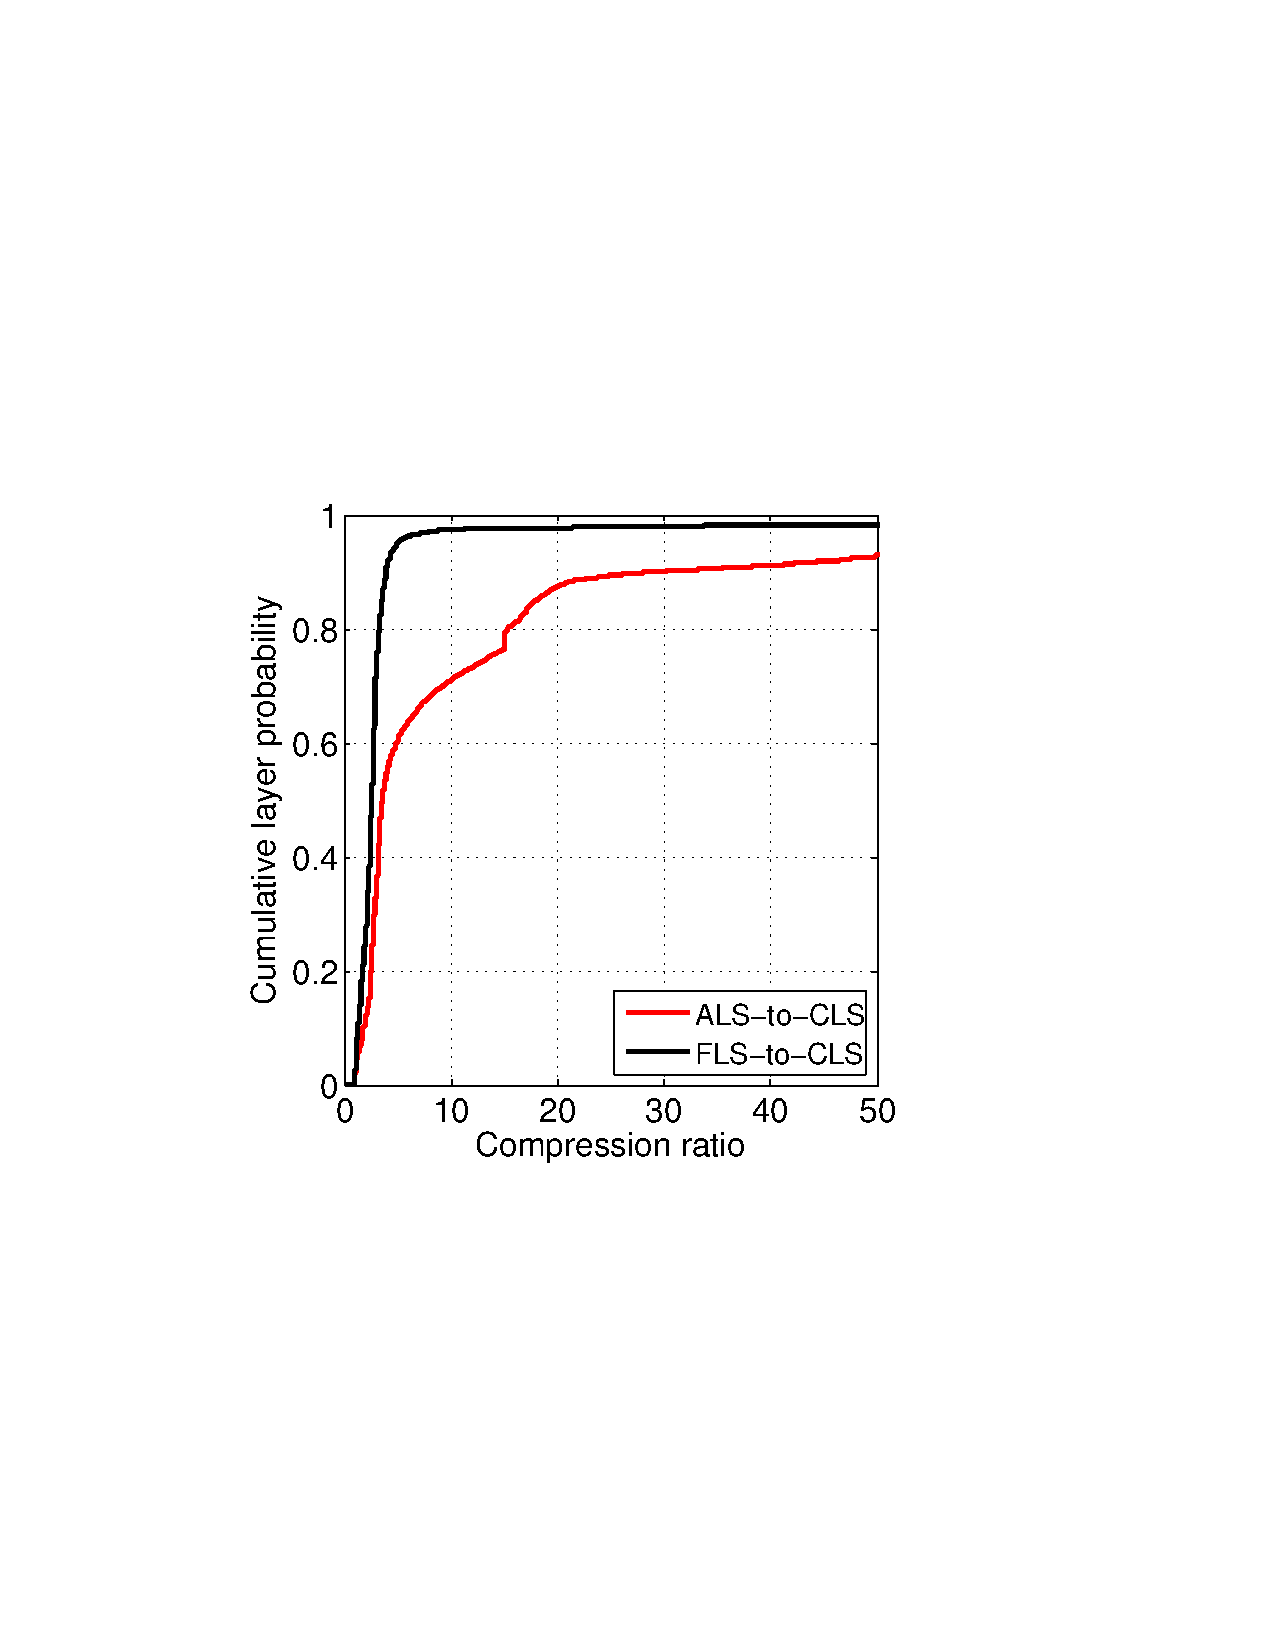
\includegraphics[width=0.23\textwidth]{graphs/cdf_compression_ratio.pdf}
	}
	\subfigure[Histogram of comp. ratios]{\label{fig_his_compression_ratio}
		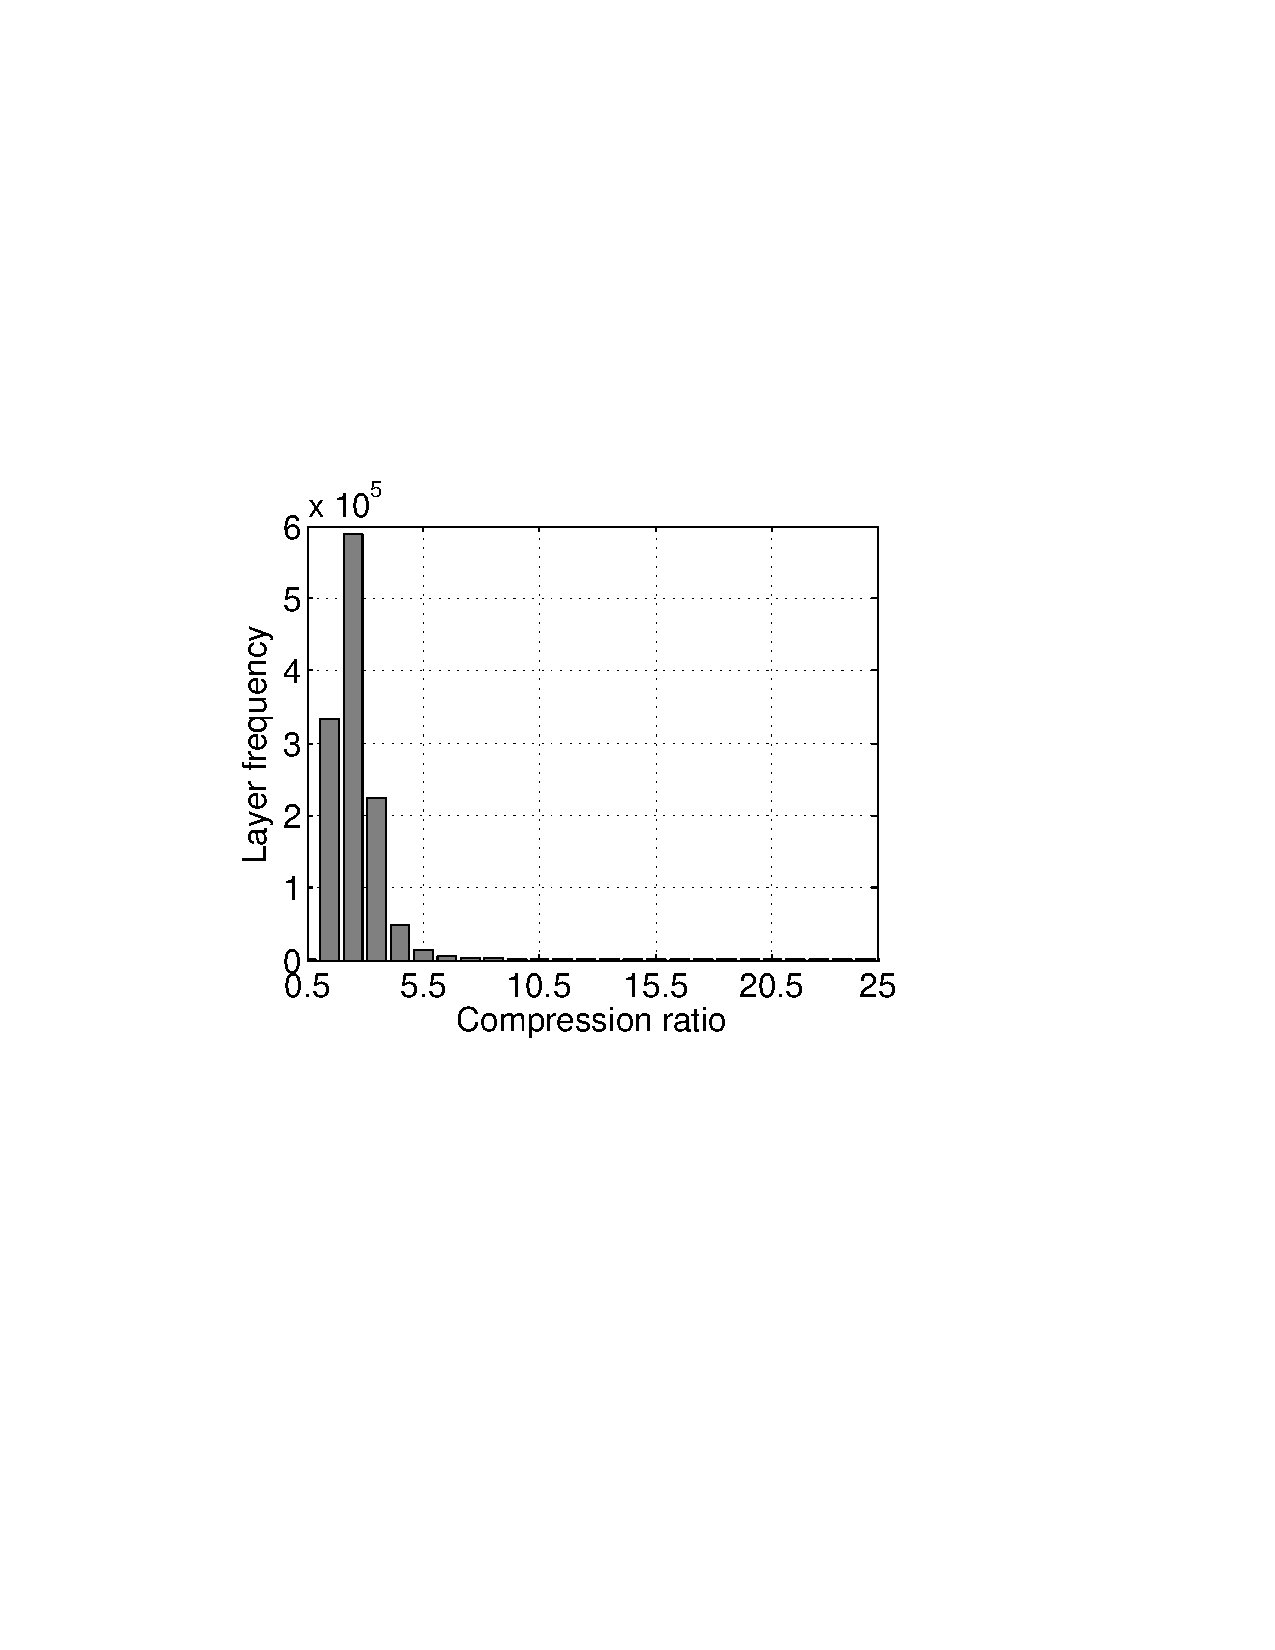
\includegraphics[width=0.223\textwidth]{graphs/his_compression_ratio.pdf}
	}
	\caption{Layer compression ratio distribution
	%\vcomment{Different colors are used in figure (a) and (b) FLS/CLS\nancomment{will address later}}
	}
	\label{fig-compression-ratio}
\end{figure}


%\paragraph{Layer compression ratios}

To further study the sizes and the impact of compression, we calculate
the FLS-to-CLS compression ratios (see Figure~\ref{fig_cdf_compression_ratio}).
%
%The ALS-to-CLS ratio is generally greater than the FLS-to-CLS ratio
%because small files in layers get larger when combined in a tar archive.
%
90\% of layers have a  CLS-to-FLS ratio less than 4 and the median
compression ratio is 2.6. The largest compression ratio is 1026.
%
%Half of the layers have a compression ratio (both ALS-to-CLS and
%FLS-to-CLS) around 3.
%
%
%The maximum FLS-to-CLS is 512,930 and maximum ALS-to-CLS is 1026.
%
Looking at the histogram (see Figure~\ref{fig_his_compression_ratio}), we see
that around 600,000 layers have a compression ratio of between 1.5 and 2.5 while more than
300,000 between 0.5 and 1.5.
%
%Two peaks in the graph correspond to 587,000 layers that have the FLS-to-CLS ratio of 3
%and 331,000 layers that have the ALS-to-CLS ratio of 3.

Our size analysis reveals an interesting trade-off. Compression is computationally
expensive and is one of the major sources of latency when pulling an image from Docker Hub.
As the majority of layers is small and has low compression ratios, it can
be beneficial to store small layers uncompressed in the registry to reduce pull latencies.

%%%%%%%%%%%%%%%%%%%%%%%%%%%%%%%%%%%%%%%%%%%%%%%%%%%%%%%%%%%%%%%%%%%%%

\begin{figure}
	\centering
	\begin{minipage}{0.23\textwidth}
		\centering
		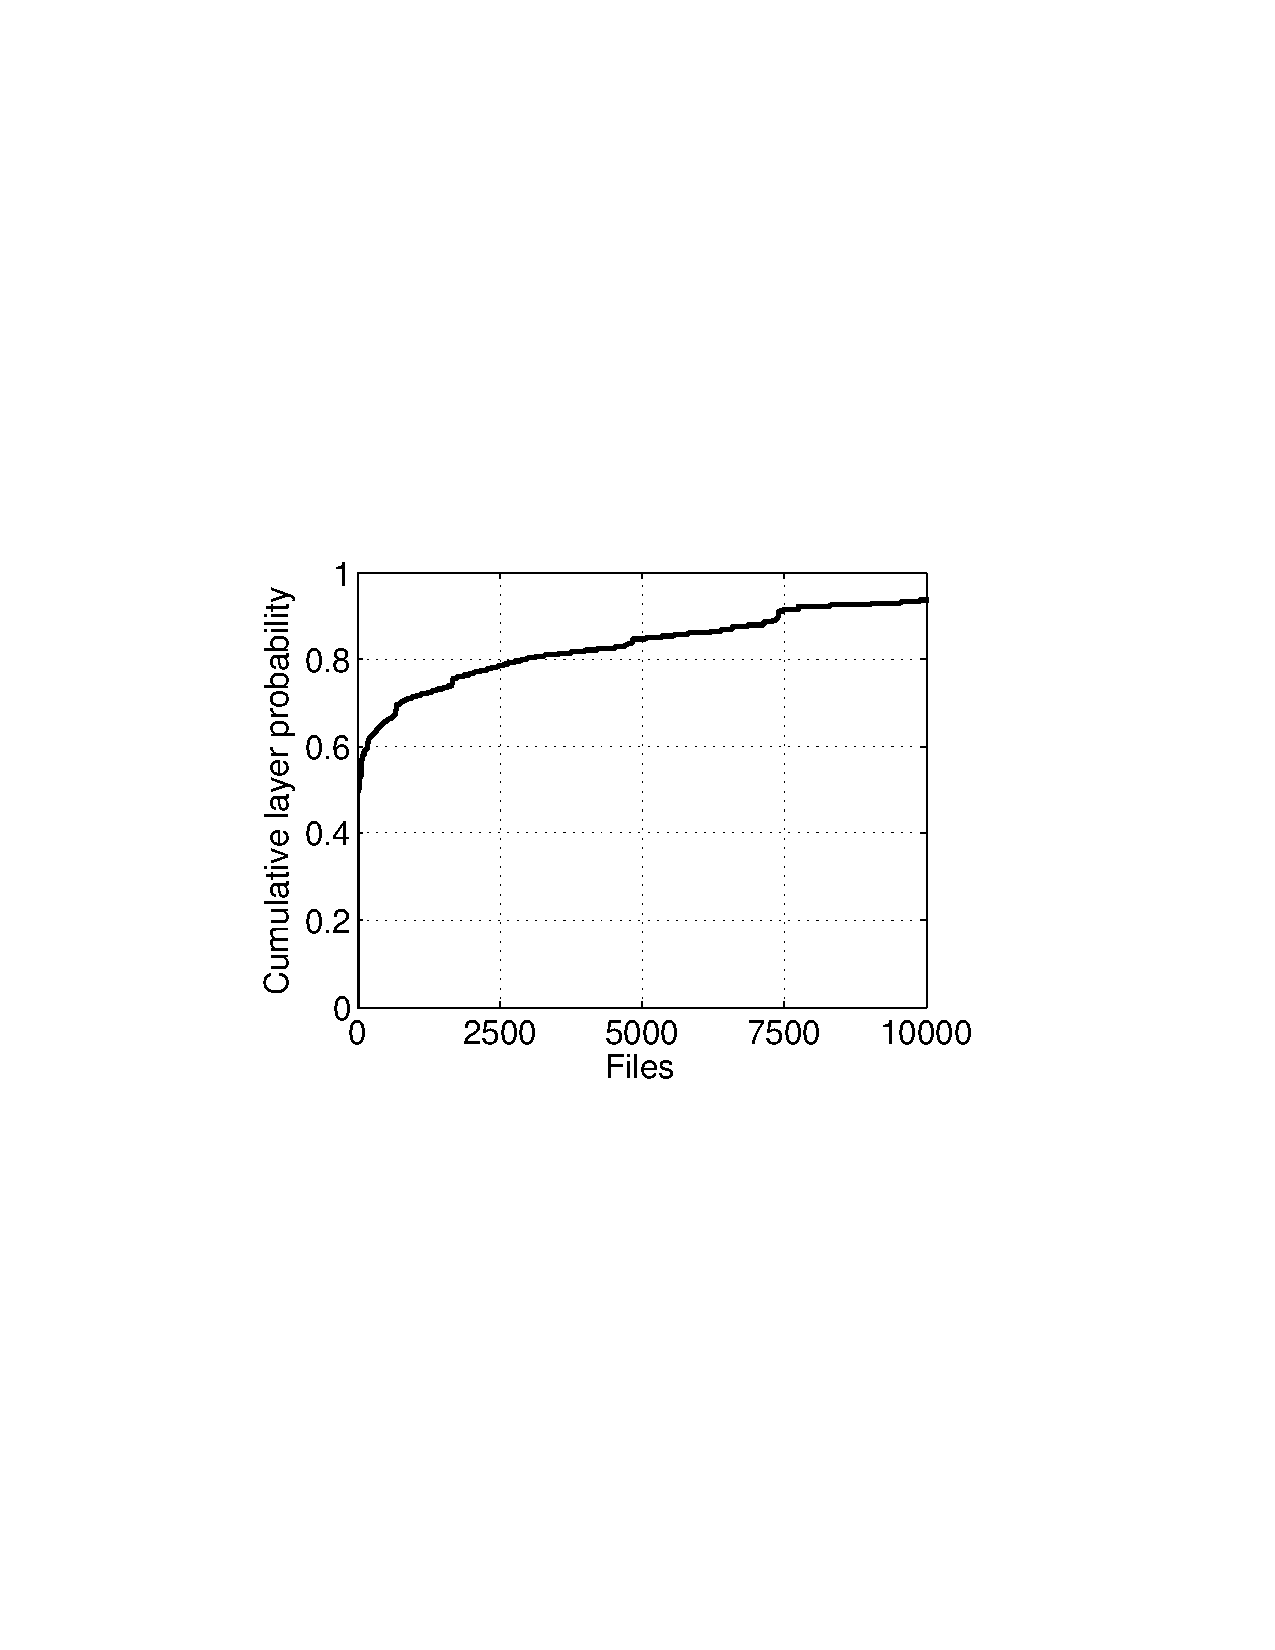
\includegraphics[width=1\textwidth]{graphs/file_cnt.pdf}
		\caption{File count distr.}
		\label{fig_file_cnt}
	\end{minipage}
	\begin{minipage}{0.23\textwidth}
		\centering
		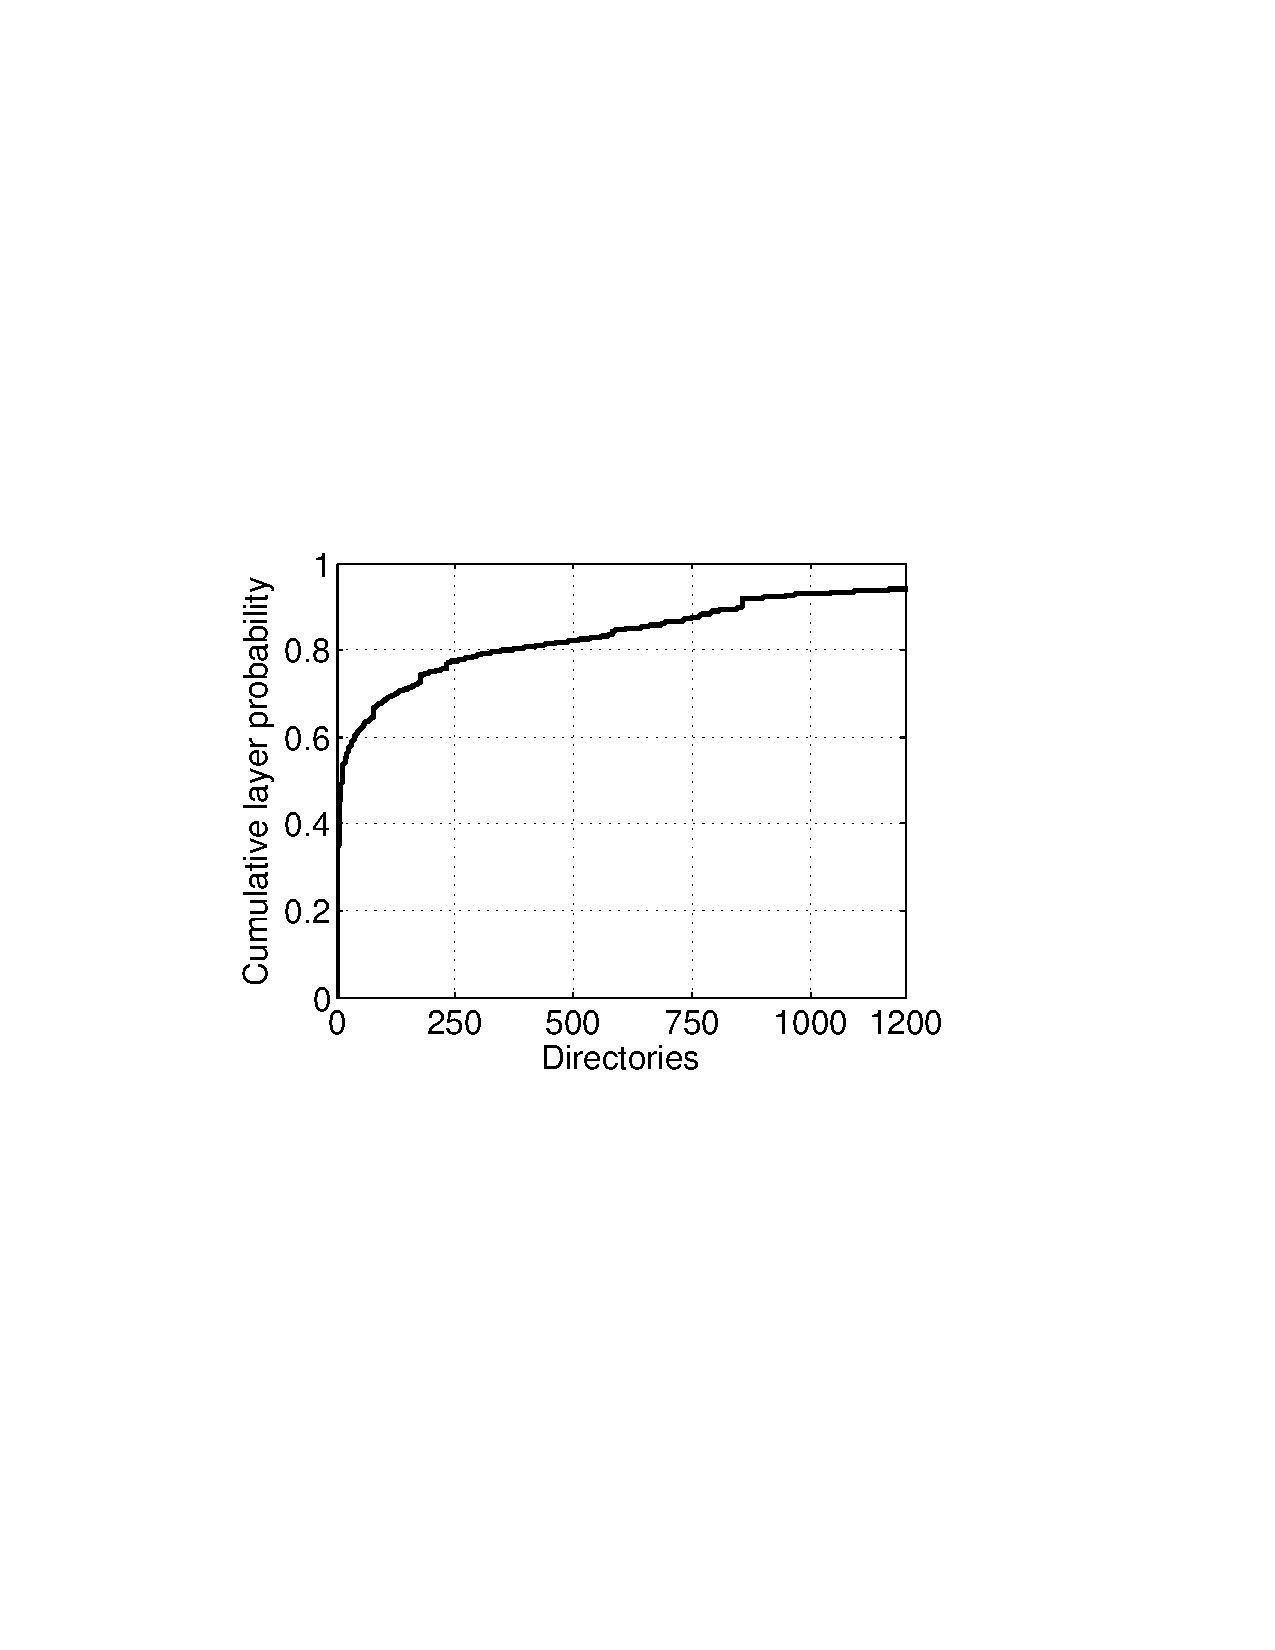
\includegraphics[width=1\textwidth]{graphs/dir_cnt.pdf}
		\caption{Dir. count distr.
		%\vcomment{Let's make thise figure subfigures.}
		}
		\label{fig_dir_cnt}
	\end{minipage}%
\end{figure}
%

\paragraph{File and directory counts}

Next, we look at file and directory metrics in layers.
Figure~\ref{fig_file_cnt} and~\ref{fig_dir_cnt} show the CDFs of file
and directory counts in all layers, respectively.
%
The results show that 90\% of layers contain less than 7,410 files while half
of the layers have less than 30 files.
%
We also found that 27\% of the layers only have a single file while 7\% even showed
no files at all. We currently do not know the exact reason for the empty layers but
plan to investigate their corresponding images in the future. On the other hand,
the largest layer contains 826,196 files which was part of a Debian image.
%
%The average is 2,200.
%
For directories, 90\% of the layers have less than 826 directories and half of the layers consist
of less than 11 directories. We again observe a wide range with a minimum of a single directory
and a maximum of 111,940. The layer with the most directories was part of
the \textit{conjurinc/developer-quiz} image.

%\paragraph{Directory depths}

%After extracting and unpacking gzip compressed layer archival files,
Besides the count, we also calculate the maximum directory depth for every layer
(see Figure~\ref{fig_layer_depth}).
%
Around 90\% of all layers have a directory depth less than 10
while for 50\%  of the layers, the directory depth is less than 4. 
%
The most frequent directory depth is 3 with 313,000 layers showing
this depth value (see Figure~\ref{fig_hist_layer_depth}.
%
%About 313,000 layers' layer directory depth is 3, which is the peak value in
%the figure.
%
%The maximum repeat count is 444 while the median is 4. The average is ~5.

This analysis shows that the majority of layers consists only of a small number
of files and does not contain deeply nested directory hierarchies. Hence, except
a few outliers, layers do not require a large amount of metadata from the storage
system.

\begin{figure}[!t]
	\centering
	\subfigure[CDF of layers by layer directory depth]{\label{fig_layer_depth}
		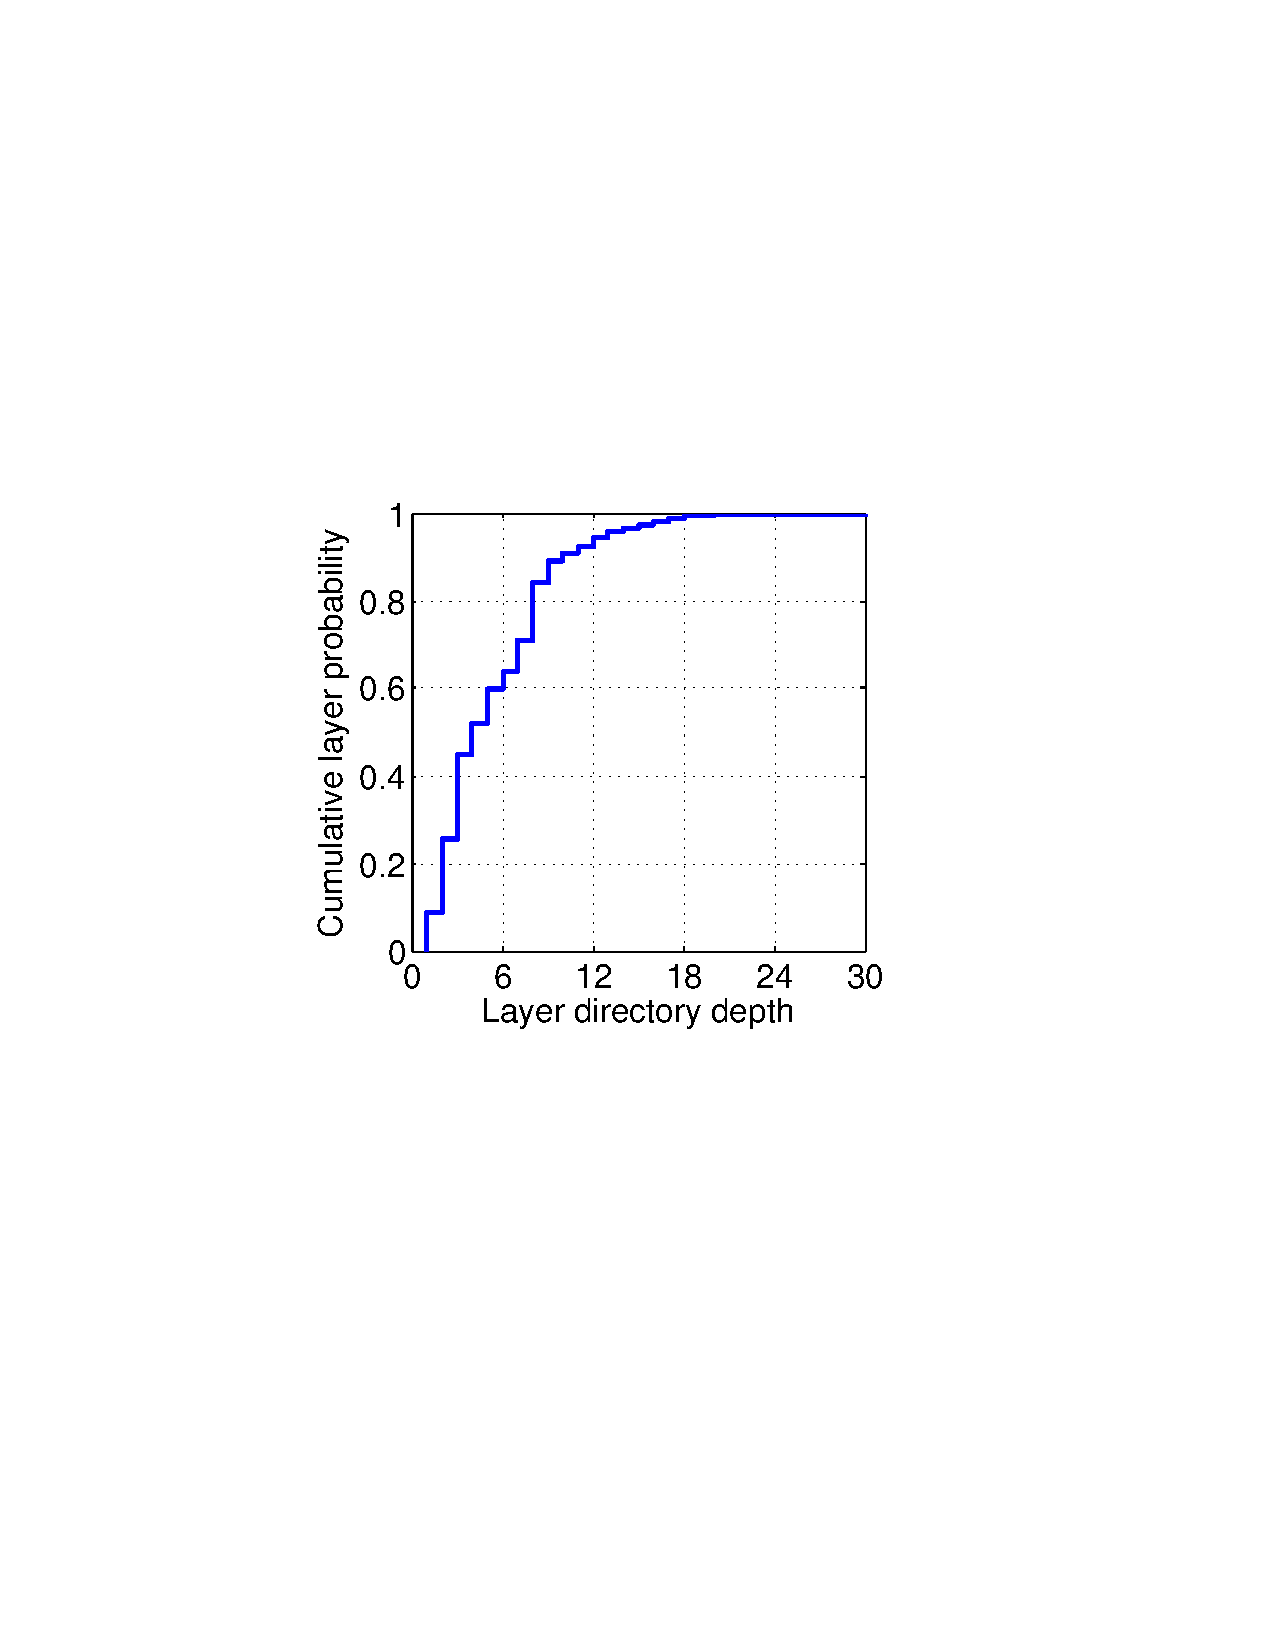
\includegraphics[width=0.23\textwidth]{graphs/layer_depth.pdf}
	}
	\subfigure[Histogram of layers by layer directory depth]{\label{fig_hist_layer_depth}
		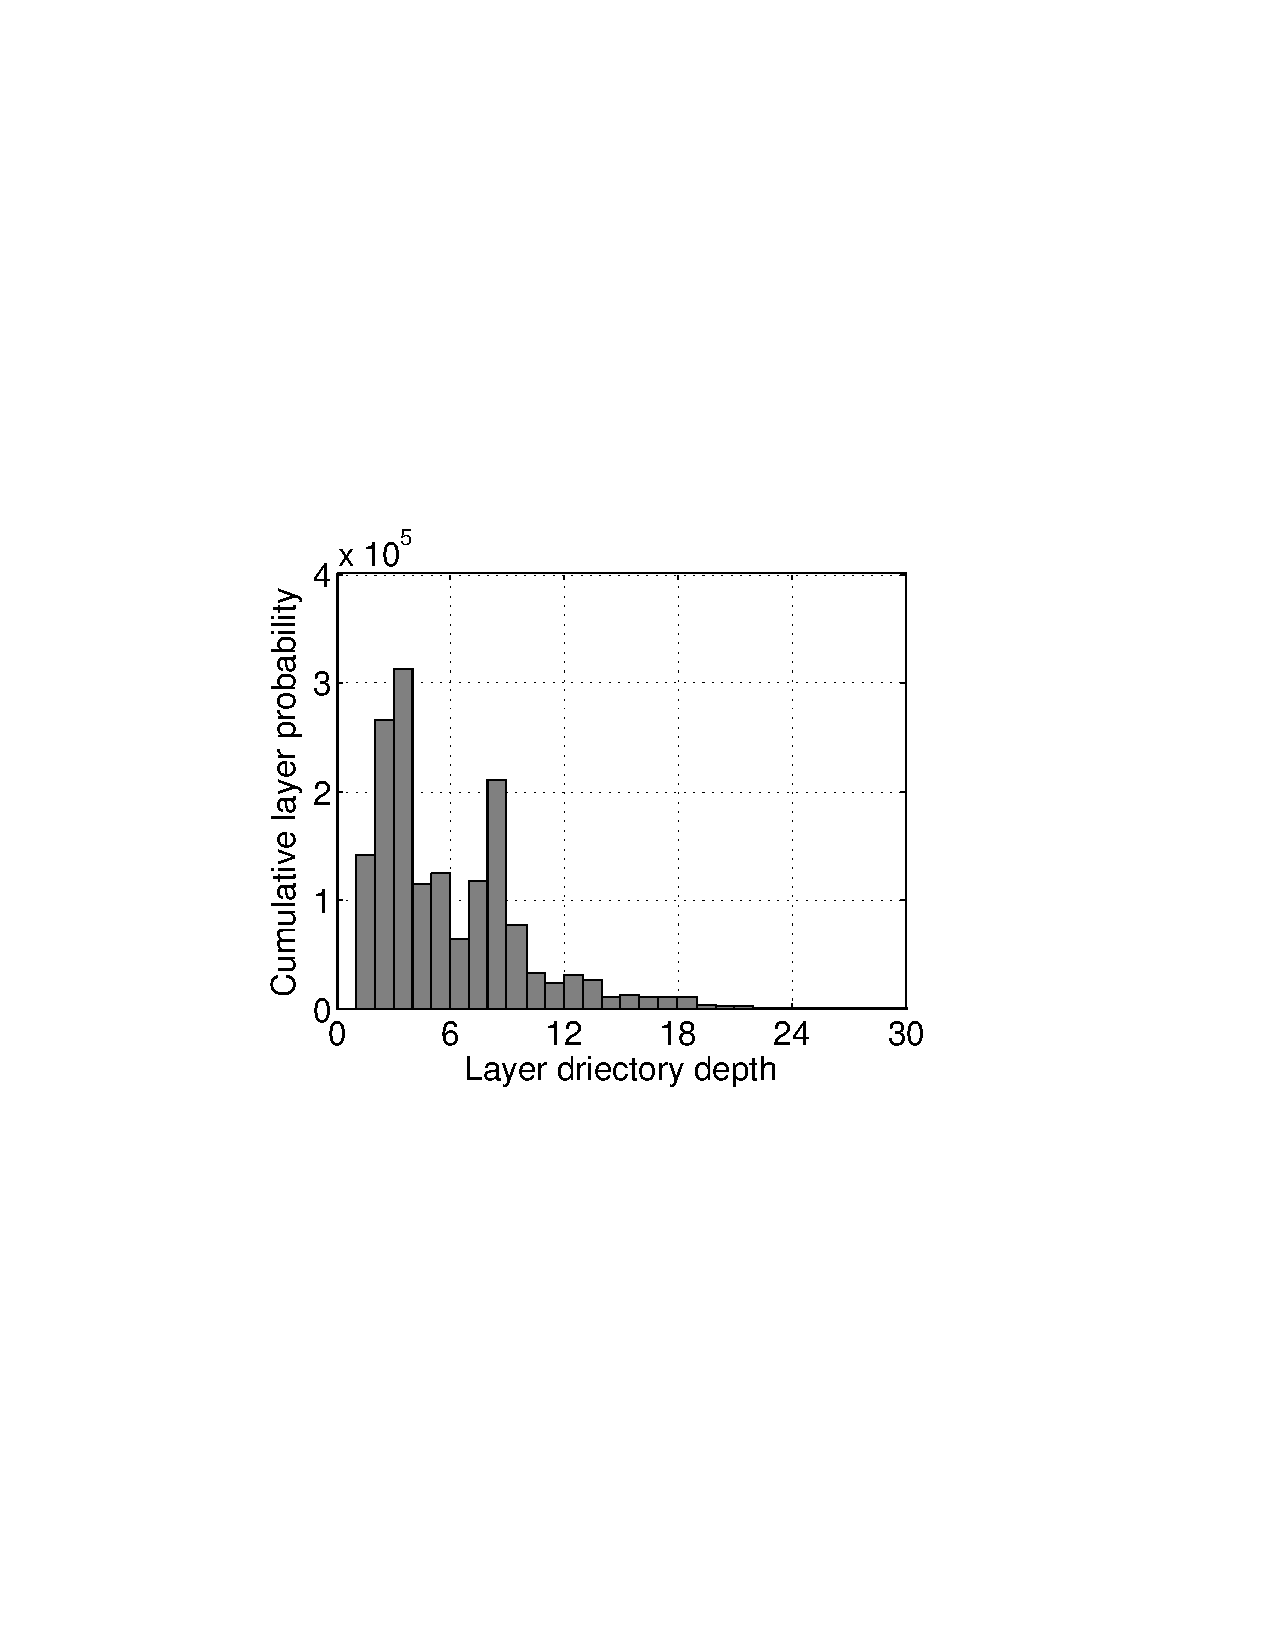
\includegraphics[width=0.22\textwidth]{graphs/hist_layer_depth.pdf}
	}
	\caption{Layer directory depth distribution}
	\label{fig-layer-dir}
\end{figure}
